\section{Methods for eliciting the selected eye tracking parameters}
\label{sec:fwkmethods}

As described preliminarily during the literature review of the single eye parameter, each eye parameter of interest can be measured by a series of methods (Tab.~\ref{tab:methodsliterature}), which are here summarized together with guidelines for setting up the experiment stimuli and procedure.

\begin{table}[h]
  \centering
  \begin{tabular}{c|c}
    Age  & IQ  \\ 
    \hline
    10   & 100 \\
    20   & 100 \\
    30   & 150
  \end{tabular}
  \caption{Summary of the methods reported in literature for the eye parameters of interest.}
  \label{tab:methodsliterature}
\end{table}



\subsection{Smooth pursuit assessment}
\label{sec:fwksmoothpursuit}

Here it follows a summary of the recommendations (and the rationale behind them) provided by \cite{smyrnis2008guidelines} in function of what emerged from literature about the use of smooth pursuit tasks for testing oculomotor functions for early ASD detection on the target children.
The sampling frequency of the eye tracking apparatus should be at least 200 Hz.

The open-loop condition can be assessed by using a step ramp task, in which the stimulus makes a sudden movement (the “step”) to a peripheral location of the visual field, then moves with constant speed in the opposite direction (the “ramp”) and finally stops (Fig.~\ref{fig:steprampscheme}). This task is useful for measuring the initial acceleration of the eye, which is aimed to catch up with the stimulus after the step when the ramp begins. The study from \cite{takarae2004smoothpursuit} used this method, along with pure ramp and oscillating target tasks. However, they observed ASDg showing lower open-loop pursuit gain in the initial catch-up saccades only during the step-ramp task, while in the other tasks only the closed-loop gain was reduced. Therefore only the step ramp task is taken into consideration for this framework.

\begin{figure}[h]
  \centering
  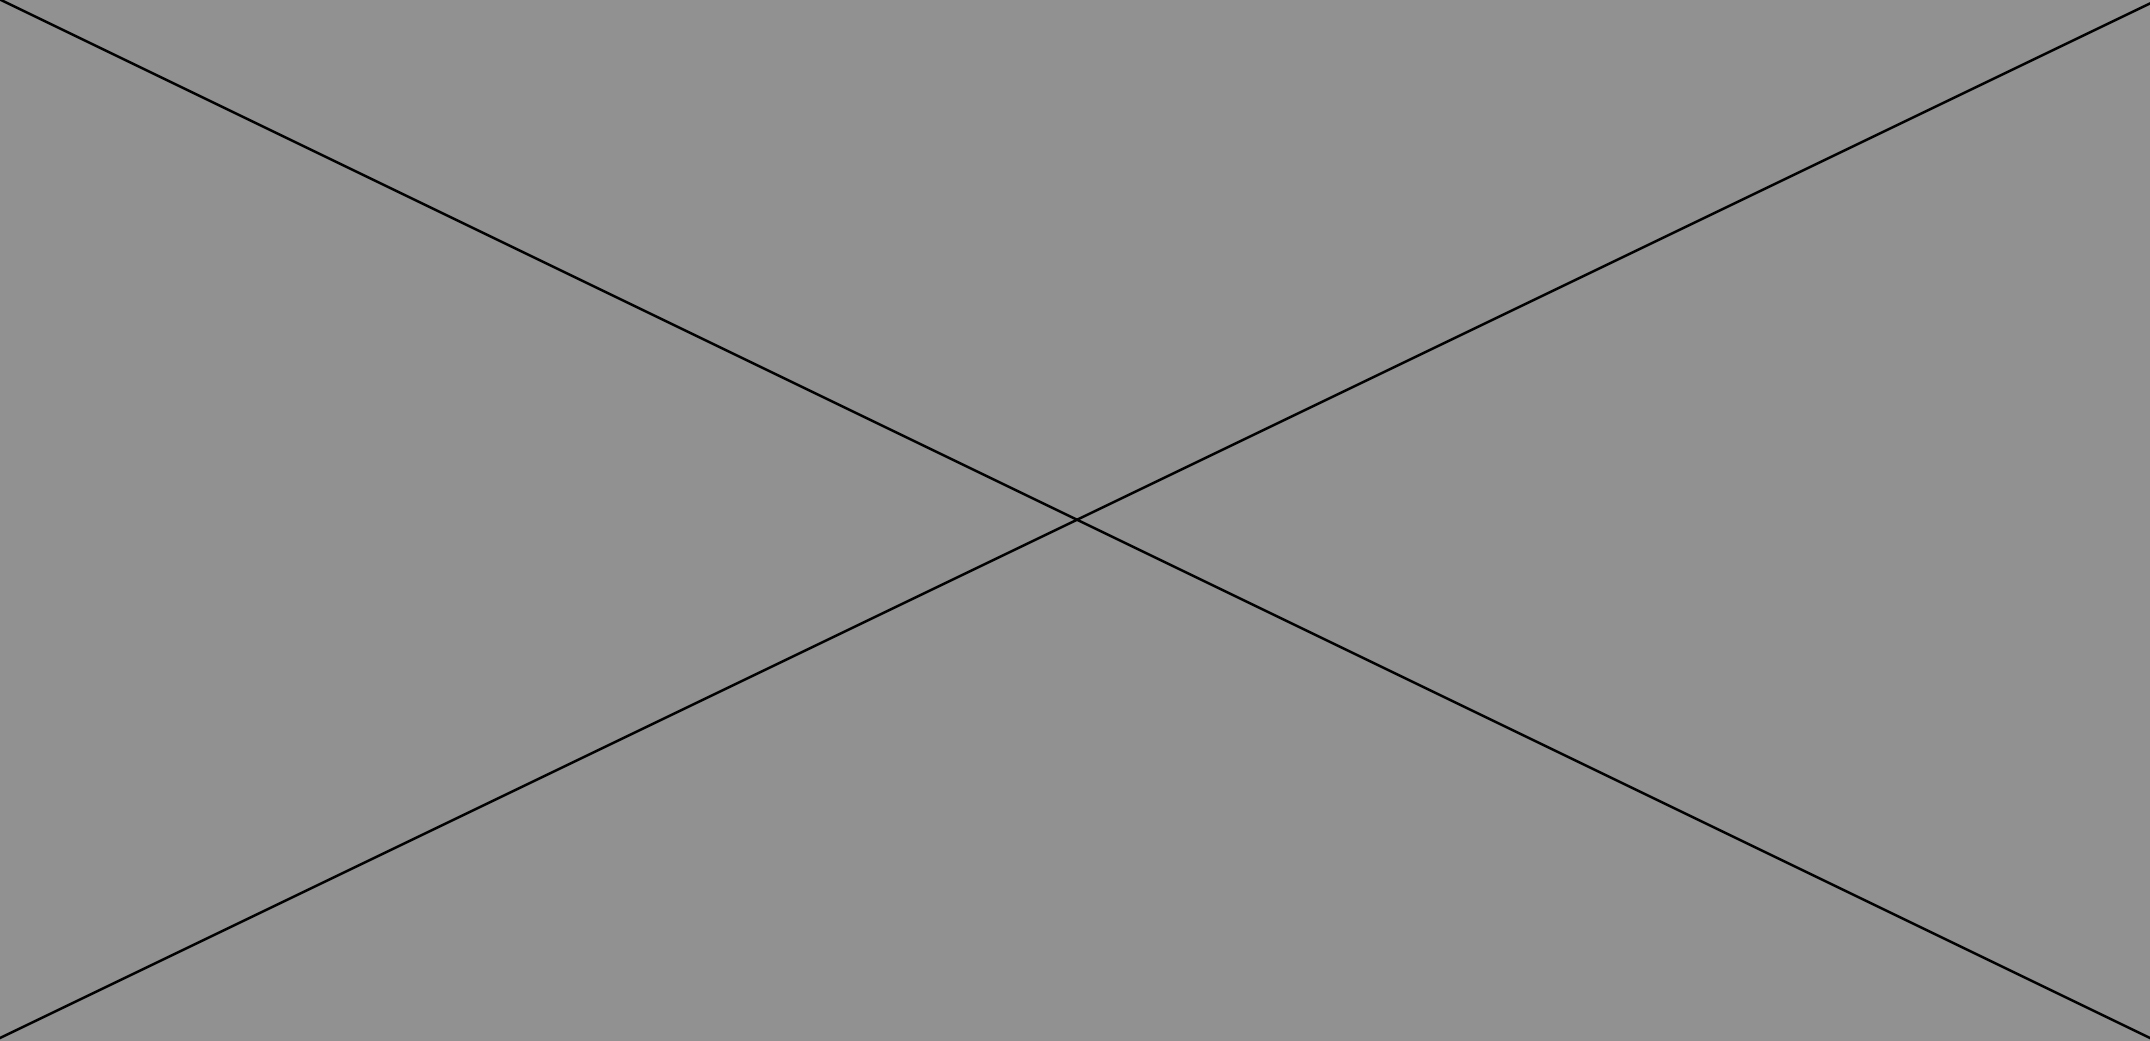
\includegraphics[width=.5\textwidth]{figures/placeholderImg.jpg}
  \caption[pursuit measurements ASDg]{Schematic representation of step ramp task. The solid line represents a typical eye movement response, while the dashed line represents target movement. Image retrieved from \cite{takarae2004smoothpursuit}}
  \label{fig:steprampscheme}
\end{figure}

The preferable closed-loop condition use triangular motion, ranging in speed from \(\leq\)10 deg/s and the high end of 20–30 deg/s. However, the relevant studies reviewed by \cite{johnson2016review} use sinusoidal motion stimuli, and the study from \cite{vonhofsten1997smoothpursuit} uses both sinusoidal and triangular motion stimuli. This latter study provides measurements done on TDg infants, which can be useful to compare with ASDg development patterns. Therefore, also a closed loop condition using sinusoidal motion should be tested, at the same conditions of the triangular motion one. As \cite{smyrnis2008guidelines} explains, different stimulus profiles lead to different interpretations of the results:
\begin{itemize}
    \item In the sinusoidal velocity profile the target speed varies continuously in a sinusoid fashion determined by a single frequency, and this stimulus is useful to determine the acceleration saturation of smooth pursuit to predictable target motion and is also for measuring overall pursuit performance. Since the target speed varies continuously (ranging from 0 deg/s to \textit{n} deg/s), it is not directly comparable to the speed for triangular or trapezoidal target motion.
    \item In the triangular velocity profile the target moves with constant speed and changes direction abruptly at the end of each run, and it is useful for for determining the steady state pursuit velocity and velocity saturation. This profile is not useful for determining global pursuit performance, since the strategy through which the subjects recover the pursuit after the abrupt change of target direction can vary considerably.
    \item Trapezoidal velocity profiles have not been found in the background literature, so they are not considered in this framework.
\end{itemize}

Given the young age of the target subjects for the framework, keeping their attention focused on the moving target during smooth pursuit tasks can be a challenge. As \cite{smyrnis2008guidelines} highlights, manipulating the shape of the target in order to facilitate performance of the task by driving the individual’s attention to the stimulus, however it makes difficult to evaluate the impact of the target transformation and compare the results across studies, making even harder to identify possible parameters as endophenotypes. Therefore, the shape of the target needs to be interesting enough to the infant without changing/transforming during the smooth pursuit task, in order to keep the stimuli stable and at the same time encourage the subjects to keep following the target without further prompting.

The task duration for sinusoidal and triangular motion stimuli is determined by the number of cycles. A cycle is completed when the target moves towards one direction and then goes back to reach the starting point. The more cycles are performed by the subject, the more measurements of pursuit performance are available, resulting in a more reliable measurement. However, it is not clear from literature what is the minimum number of cycles for each stimulus speed. There might be an unknown balance between having a reliable measurement and adding practice effects, due to the subjects’ habituation to the task. \cite{smyrnis2008guidelines} advices at least five, which is similar to what  \cite{vonhofsten1997smoothpursuit} did in their experiments.



\subsection{Saccades assessment}
\label{sec:fwksaccades}

\cite{johnson2016review} explain the need to distinguish between visually-guided saccades from volitional saccades, due to the involvement of different cortical, subcortical and cerebellar networks when performing each class of eye movement. In visually-guided saccade tasks, participants are presented with a central fixation target and then a peripheral target appears concomitantly to the central fixation target disappearing.

\cite{brenner2007visualsearch} describe visually-guided saccades also as reflexive, non-predictive. Visually-guided saccades tasks are therefore designed to assess target-elicited saccades, which are driven by exogenous stimuli. These tasks are used in opposition to intentional-saccade tasks (e.g. memory-guided, predictive, anti-saccade tasks). \cite{johnson2016review} add that anti-saccade task is frequently used to examine top-down control of saccades, since they ask the participant to suppress a reflexive saccade to a visual target and to make a volitional saccade in the equal opposite position.

Due to their nature, antisaccade tasks (but also the other kinds of volitional saccades) are impractical to do with small children, since the researcher would need to instruct the child to purposely not look at the target and to look at the opposite direction. Young children may be unable or unwilling to follow verbal instructions to look to specific locations on the screen \citep{sasson2012children}. Therefore, antisaccade tasks are not considered in this framework.

Summarizing from \cite{zalla2016saccades}, the Step, Gap and Overlap paradigms are well-validated visually guided saccade tasks:
\begin{itemize}
    \item Step paradigm: the subject fixates a central fixation target and as soon as it disappears a lateral target appears, requiring the subject to make a lateral saccade. When the lateral target disappears a new central fixation target is presented, starting a new trial. 
    \item Gap paradigm: follows the same routine of the Step paradigm, but the central fixation target disappears before the onset of the peripheral stimulus.
    \item Overlap paradigm: follows the same routine of the Step paradigm, but the central fixation target remains on display when the peripheral stimulus is shown.
\end{itemize}

Gap/Overlap paradigms are useful to assess attention shift and disengagement between the central and the peripheral targets, by analyzing saccade latency (basically the response time). 

Here it follows the discussion around the recommendations for assessing saccades from Smyrnis (2008) in function of early ASD detection on the target children.
The sampling frequency of the eye tracking apparatus should be at least 200 Hz.

It is better to avoid complex stimuli and gap or precues between stimuli which change the performance. Therefore, the peripheral target onset needs to occur synchronously with the central fixation offset (step paradigm), not before (introducing overlap) or after (introducing gap).

Stimulus should appear both at right and left directions and at multiple amplitudes within the range of 10 deg, avoiding targets appearing too close to the central fixation target (\(\leq\) 2 deg) or too far (\textgreater 15 deg). \cite{johnson2016review} report that the standard deviation of saccade gain is expected to be significantly different in ASDg at target amplitudes ranging from 5 to 30 deg, therefore a compromise is to show targets between 5 to 15 deg of distance from the central target.

A sufficient number of trials can be within 30 and 100, but not greater in order to avoid practice and fatigue effects.
